%  CONFIGURE NEWcitep SINGLE-PAGE FORMAT

\onecolumn % go back to one column
%\fancyhead{} % make sure we get no headers
\renewcommand{\floatpagefraction}{0.1}
%\lfoot[\bSupInf]{\dAuthor}
%\rfoot[\dAuthor]{\cSupInf}
\newpage

%\captionsetup*{format=largeformat} % make figure legend slightly larger than in the paper
\setcounter{figure}{0} % reset figure counter for Supp. Figures
\setcounter{equation}{0} % reset equation counter for Supp. Equations
%\setcounter{page}{1} % reset page count
%\makeatletter
%\renewcommand{\thefigure}{S\@arabic\c@figure} % make Figure legend start with Figure S
%\makeatother
%\def\theequation{S\arabic{equation}}
\renewcommand{\figurename}{Supplementary Figure}

%  MAIN TEXT

\newpage
\section*{Supplementary Information}

%%%%%%%%%%%%%%%%%%%%%%%%%%%%%%%%%%%%%%%%%%%%%%%%%%%%%%%%%%%%%%%%%%%%%%%%%%%%%%%%
%
% Supp fig 1: Percent of explained loci
%
%%%%%%%%%%%%%%%%%%%%%%%%%%%%%%%%%%%%%%%%%%%%%%%%%%%%%%%%%%%%%%%%%%%%%%%%%%%%%%%%

\begin{figure}[!tbp]
    \centering
    \includegraphics[width=\textwidth]{\floatRelativePath/cmpt_perc_tophits_eqtl.py/subplots.png}

    \caption{}
%
\end{figure}

%%%%%%%%%%%%%%%%%%%%%%%%%%%%%%%%%%%%%%%%%%%%%%%%%%%%%%%%%%%%%%%%%%%%%%%%%%%%%%%%
%
% Fig 2: ucsc screenshots
%
%%%%%%%%%%%%%%%%%%%%%%%%%%%%%%%%%%%%%%%%%%%%%%%%%%%%%%%%%%%%%%%%%%%%%%%%%%%%%%%%

\begin{figure}[!ht]
    \centering

    \begin{subfigure}[]{0.99\textwidth}
        \textbf{a}
        \\
        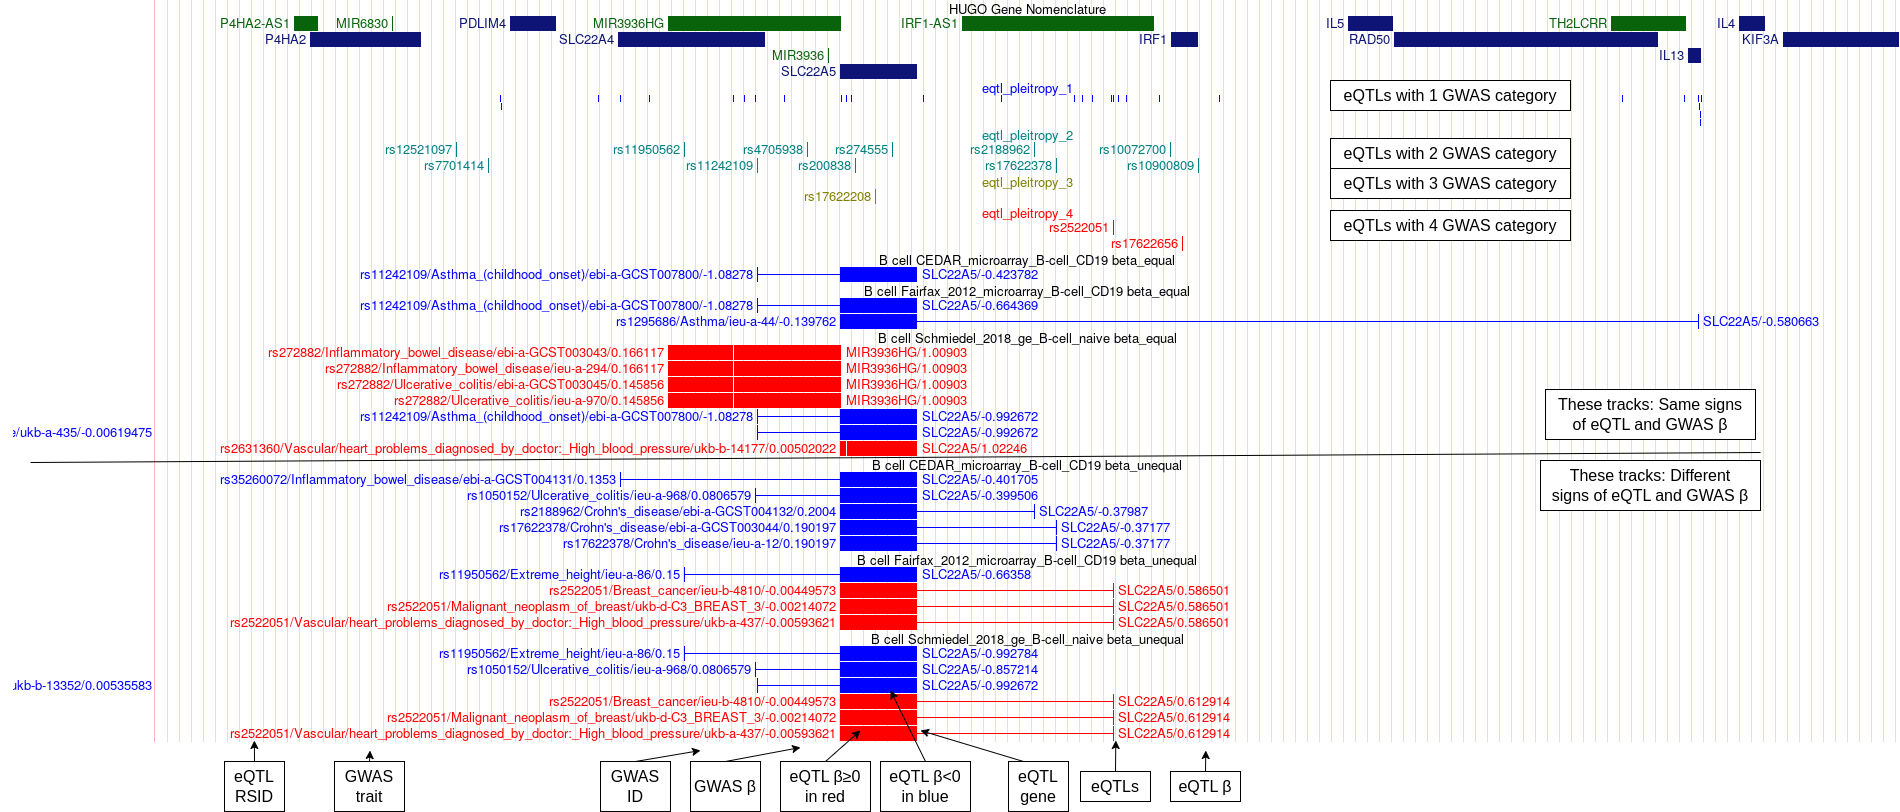
\includegraphics[width=\textwidth]{fig/ucsc_gwas2eqtl_il4_bcell_help.png}
    \end{subfigure}

    \begin{subfigure}[]{0.99\textwidth}
        \textbf{b}
        \\
        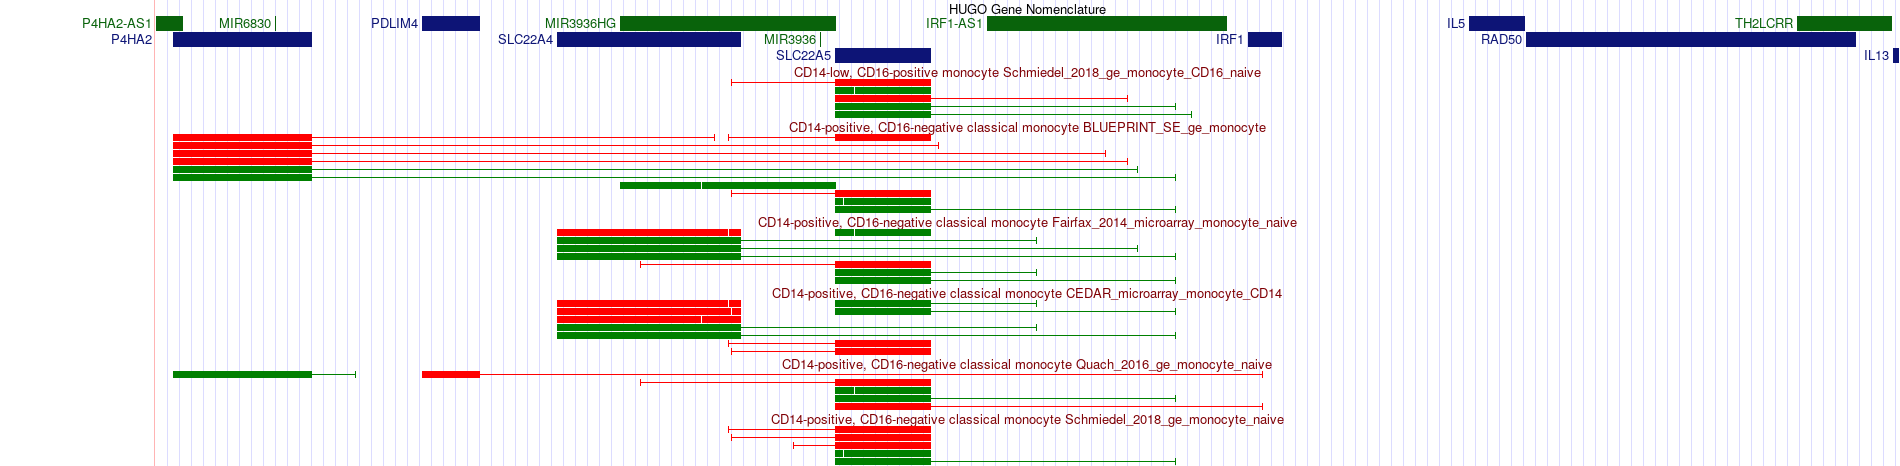
\includegraphics[width=\textwidth]{fig/ucsc_gwas2eqtl_il4_monocyte.png}
    \end{subfigure}

    \begin{subfigure}[]{0.99\textwidth}
        \textbf{c}
        \\
        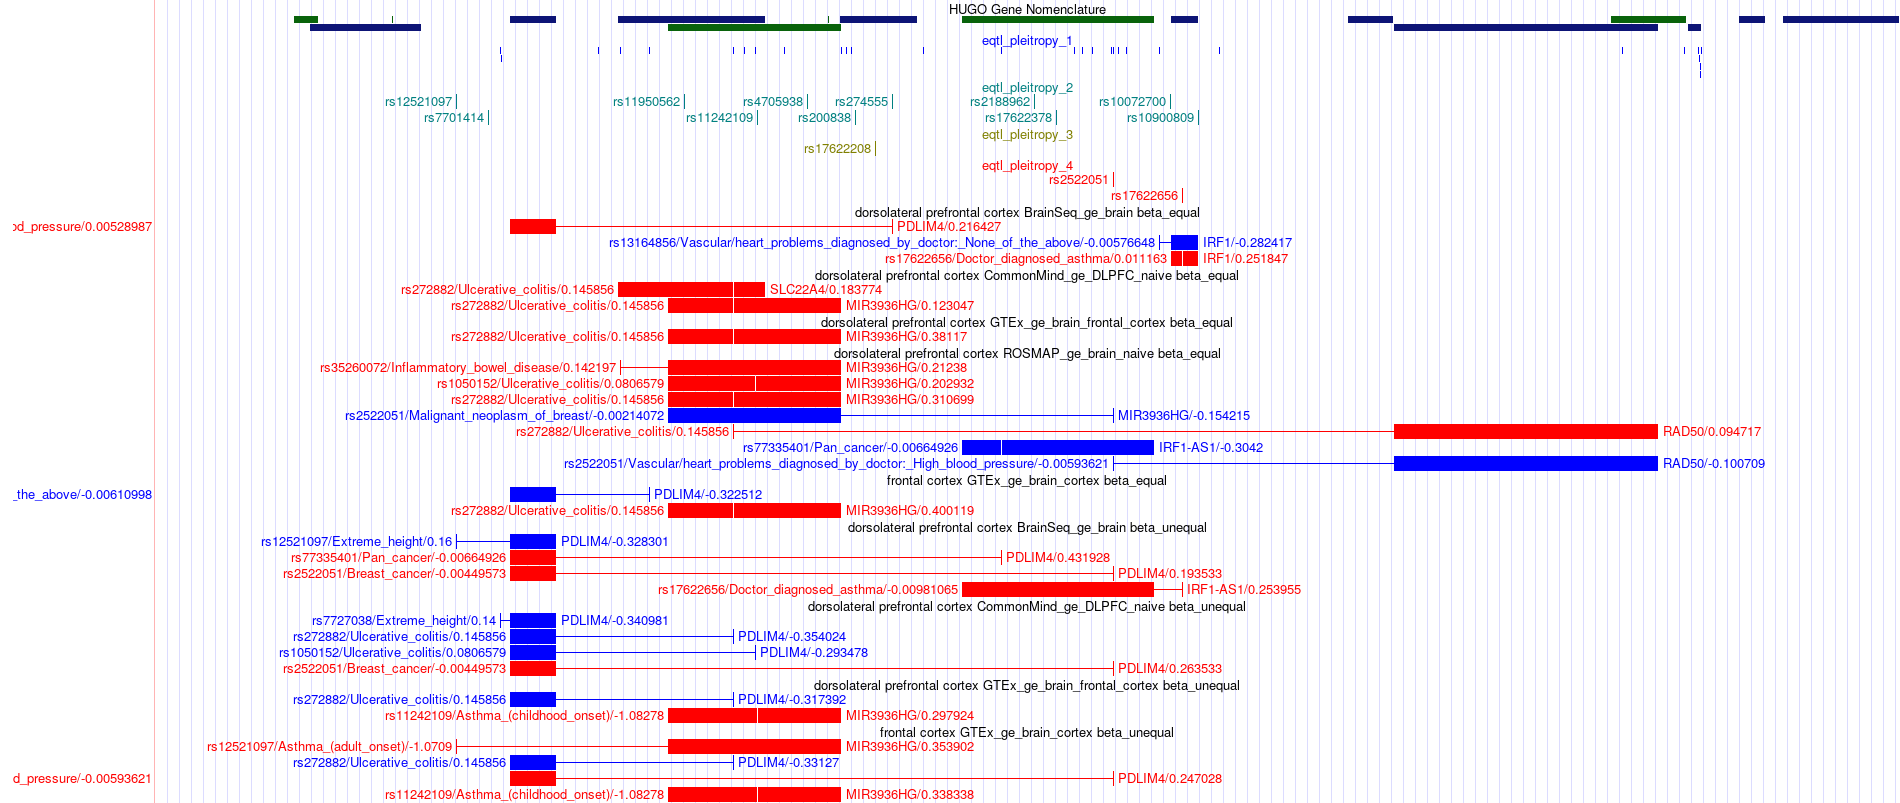
\includegraphics[width=\textwidth]{fig/ucsc_gwas2eqtl_il4_frontalcortex.png}
    \end{subfigure}

    \caption{}

\end{figure}

%%%%%%%%%%%%%%%%%%%%%%%%%%%%%%%%%%%%%%%%%%%%%%%%%%%%%%%%%%%%%%%%%%%%%%%%%%%%%%%%
%
% Fig 5: Comparison with Watanabe 2019
%
%%%%%%%%%%%%%%%%%%%%%%%%%%%%%%%%%%%%%%%%%%%%%%%%%%%%%%%%%%%%%%%%%%%%%%%%%%%%%%%%

\begin{figure}[!ht]
    %
    \centering
    %
    \begin{subfigure}[]{.49\textwidth}
        \textbf{a}
        \\
        \includegraphics[width=\textwidth]{\floatRelativePath/cmpt_count_per_rsid.py/watanabe_cat_count.png}
    \end{subfigure}
    %
    \begin{subfigure}[]{.49\textwidth}
        \textbf{b}
        \\
        \includegraphics[width=\textwidth]{\floatRelativePath/cmpt_count_per_rsid.py/watanabe_percentage.png}
    \end{subfigure}

    \caption{}

\end{figure}

%%%%%%%%%%%%%%%%%%%%%%%%%%%%%%%%%%%%%%%%%%%%%%%%%%%%%%%%%%%%%%%%%%%%%%%%%%%%%%%%
%
% Supp fig: allele frequencies
%
%%%%%%%%%%%%%%%%%%%%%%%%%%%%%%%%%%%%%%%%%%%%%%%%%%%%%%%%%%%%%%%%%%%%%%%%%%%%%%%%

\begin{figure}[!tbp]

    \begin{subfigure}[]{.32\textwidth}
        \textbf{a}
        \\
        \includegraphics[width=\textwidth]{\floatRelativePath/pltbar_x_per_gwas_cat_y_allele_freq.py/afr_af.png}
    \end{subfigure}
%
    \begin{subfigure}[]{.32\textwidth}
        \textbf{b}
        \\
        \includegraphics[width=\textwidth]{\floatRelativePath/pltbar_x_per_gwas_cat_y_allele_freq.py/amr_af.png}
    \end{subfigure}
%
    \begin{subfigure}[]{.32\textwidth}
        \textbf{c}
        \\
        \includegraphics[width=\textwidth]{\floatRelativePath/pltbar_x_per_gwas_cat_y_allele_freq.py/eas_af.png}
    \end{subfigure}

    \centering
    \begin{subfigure}[]{.32\textwidth}
        \textbf{d}
        \\
        \includegraphics[width=\textwidth]{\floatRelativePath/pltbar_x_per_gwas_cat_y_allele_freq.py/eur_af.png}
    \end{subfigure}
%
    \begin{subfigure}[]{.32\textwidth}
        \textbf{e}
        \\
        \includegraphics[width=\textwidth]{\floatRelativePath/pltbar_x_per_gwas_cat_y_allele_freq.py/sas_af.png}
    \end{subfigure}

    \caption{}

\end{figure}
